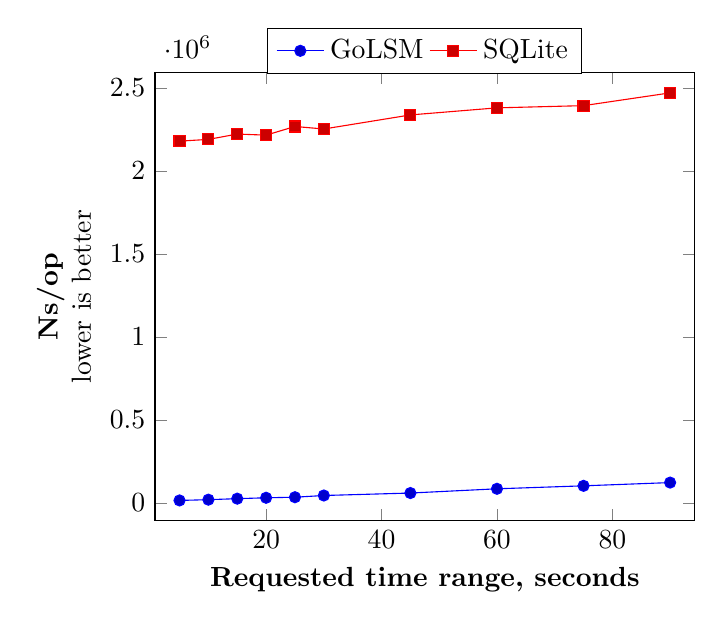
\begin{tikzpicture}
        % first provide your data as table, so later the data can
        % easily be accessed for various stuff
        \pgfplotstableread{
            x    y  z
5 14164				    2179781
10 18772			    2190392
15 24835			    2222522
20 30221			    2216021
25 33592			    2268216
30 43931			    2253056
45 58727			    2337832
60 84315			    2380516
75 102221			    2393851
90 121761			    2470748
        }{\data}
    \begin{axis}[
        x tick style={/pgf/number format/1000 sep=},
	    ylabel style={align=center},	
	    ylabel = \textbf{Ns/op}\\lower is better,
	    xlabel style={align=center},	
	    xlabel = \textbf{Requested time range, seconds},
	    enlargelimits=0.05,
	    legend style={
	        at={(0.5,1.1)}, anchor=north,legend columns=-1
	    },
    ]
        % then your `\addplot commands change to
        \addplot table [x=x,y=y] {\data};
        \addlegendentry{GoLSM}
        \addplot table [x=x,y=z] {\data};
        \addlegendentry{SQLite}
    \end{axis}
\end{tikzpicture}